\chapter{Condensed Matter XUV Transient Absorption Experiments}

\section{Statement of Contribution}
This experiment uses home-made equipment consisting of a XUV-IR Mach-Zhender interferometer, a bright XUV light source, a target chamber and an XUV photon spectrometer. The entire apparatus was designed, built and tested by Gregory Smith and Stephen Hageman. The LabView software controlling the spectrometer's detector was programmed by Kent Talbert. The vacuum system's safety system was designed and programmed by Andrew Piper. The germanium samples were grown by Dr. Yaguo Tang. Transient absorption experiments were done by Gregory Smith and Stephen Hageman. Analysis presented in this document was done by Gregory Smith. Further details on the apparatus and the relevant physics will be discussed in the main dissertation.

\section{Introduction}

\begin{figure}
	\centering
	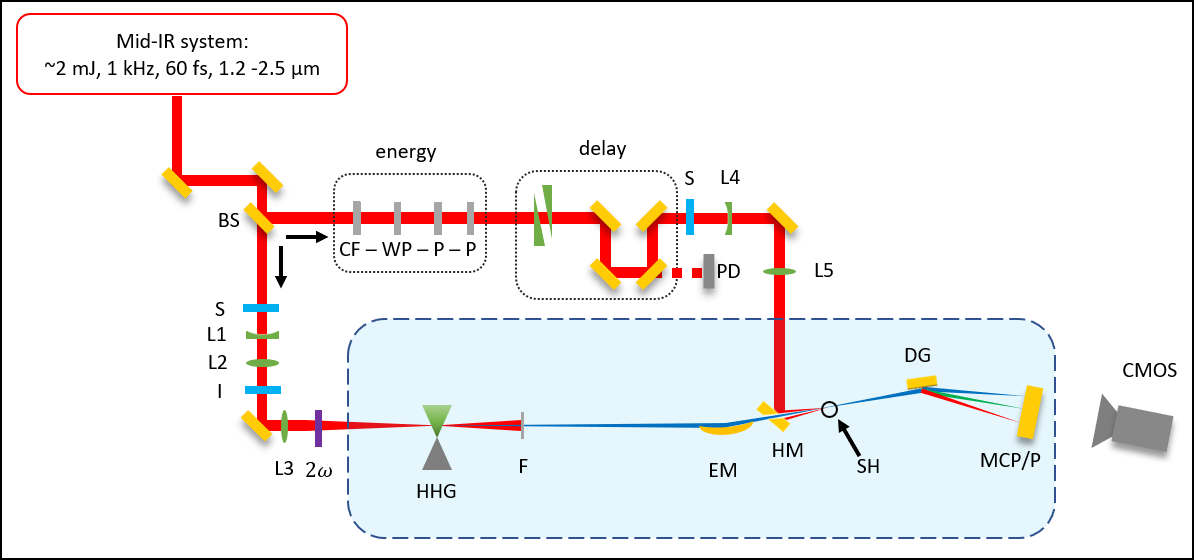
\includegraphics[width=0.95\textwidth]{figures/chap3/beamline_schematic.png}
	\caption{Schematic of the Transient Absorption BeamLine (TABLe). Blue shaded region is under vacuum. BS: beam splitter, L: lens, S: computer-controlled shutter, HHG: high harmonic generation, F: metallic filter, EM: ellipsoidal mirror, HM: hole mirror, PD: photodiode, DG: dispersive grating, MCP/P: micro-channel plate and phosphor.}
	\label{fig:beamline_schematic}
\end{figure}

\begin{figure}
	\centering
	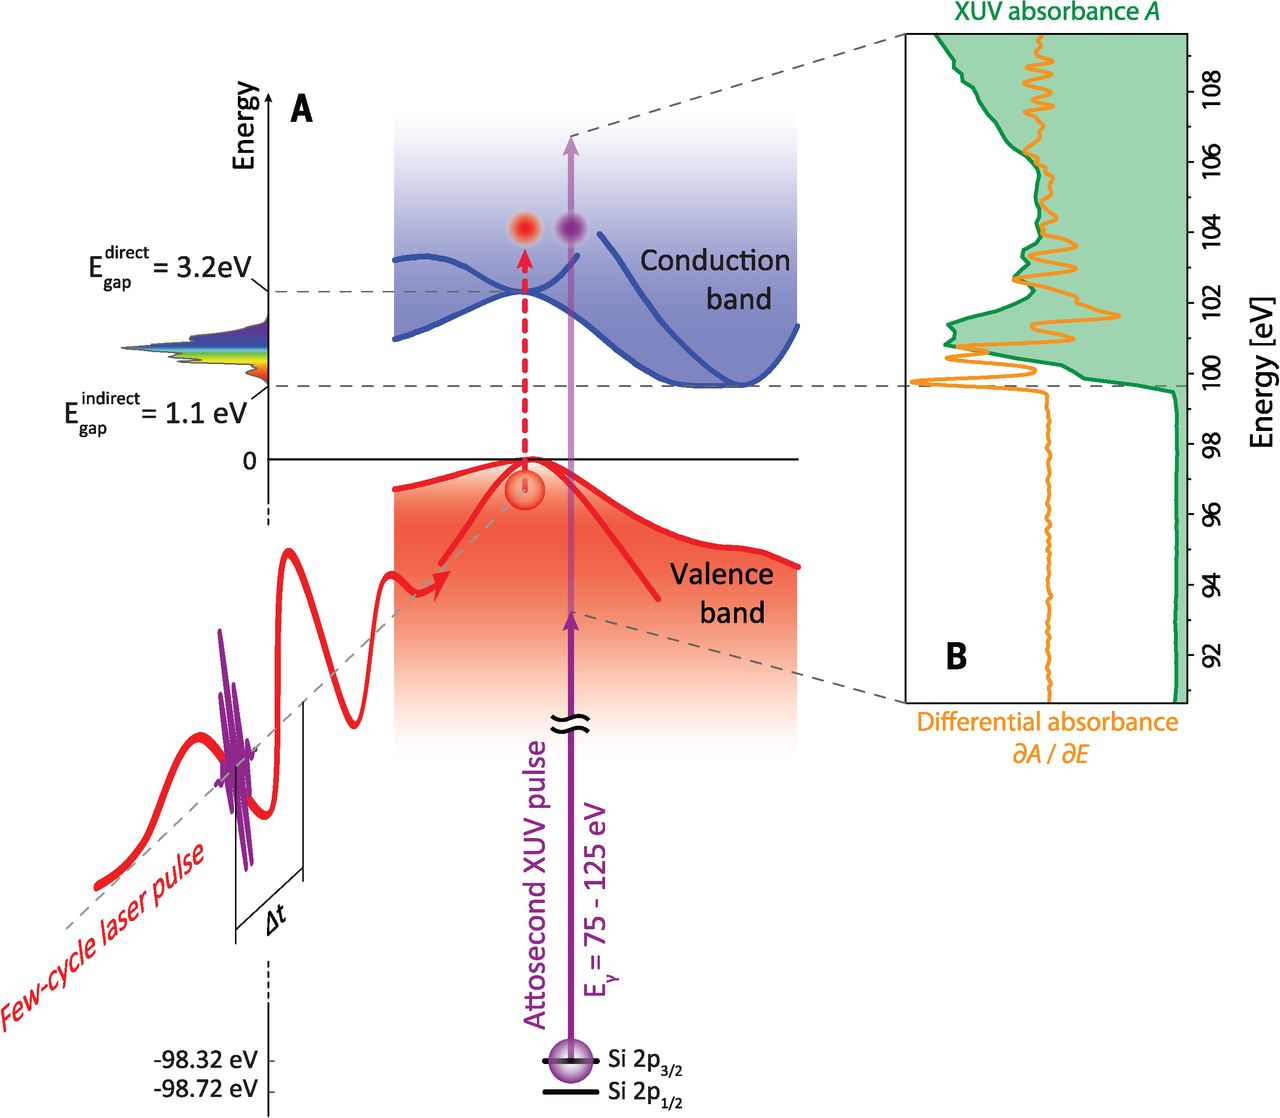
\includegraphics[width=0.75\textwidth]{figures/chap3/ATAS_Cartoon_Si_Leone.jpg}
	\caption{Schematic of an attosecond transient absorption spectroscopy (ATAS) experiment. An IR laser pulse excites electrons in the material, driving them across the band-gap. An XUV pulse passes through the sample after a delay $\Delta t$. The measured XUV absorbance is sensitive to electronic populations and states. Figure taken from \cite{schultzeAttosecondBandgapDynamics2014}.}
	\label{fig:ATAS_Cartoon_Si_Leone}
\end{figure}

We generate extreme ultraviolet (XUV) light using an extremely non-linear process called \textit{high harmonic generation} (HHG). Briefly, the XUV light source can be thought of as a frequency comb spanning from $\sim20$ eV to $\sim50$ eV. The separation between the teeth of the frequency comb is $\omega$, the frequency of our laser light. In the time domain, the XUV is a train of attosecond bursts of broadband light with an envelope of $\sim50$ fs. Due to the ionizing nature of XUV light, the entire experiment must be performed under vacuum.

The experiment is powered by a commercial mid-IR laser system (Spectra Physics Spitfire ACE, Light Conversion HE TOPAS Prime), which delivers $\sim2$ mJ at $100 - 1,000$ Hz repetition rate, $\sim65$ fs duration, $1.2 - 2.5$ $\mu$m wavelength. The output of the TOPAS is routed into a Mach-Zhender interferometer, shown in \cref{fig:beamline_schematic}. A beam splitter (BS) delivers the bulk of the pulse energy ($96\%$) to the generation arm of the interferometer, which contains the HHG source and specialized XUV focusing optics. A small percentage of TOPAS's pulse energy goes to the pump arm, which contains optics to control the pulse energy and relative delay between the two arms. The pump arm also contains a series of lenses that focus the light into the vacuum system. A silvered hole mirror (HM) combines the two arms of the interferometer collinearly. This optic is designed to allow the XUV light to pass through a clear aperture on the backside of the HM while the pump arm's IR light reflects off the front face. The interferometer is aligned so that both arms have a common focus in the target chamber.

The basic concept of an attosecond transient absorption spectroscopy (ATAS) experiment is shown in \cref{fig:ATAS_Cartoon_Si_Leone}. In this experiment, a sample is placed at the combined XUV/IR focus in a transmission (normal) geometry. An XUV photon spectrometer is placed behind the sample and the transmitted XUV spectrum $S$ is measured as a function of XUV-IR delay. The IR light is not measured by the spectrometer.

Absorption features in the spectrum correspond to photoabsorption, which drive electronic transitions. At XUV photon energies, these transitions are from a core-level state to a state near the Fermi level. Since the HHG process produces a near-continuum, the XUV light will drive nearly all allowed transitions within its bandwidth. One of the core assumptions of an ATAS experiment is that the initial core state is shielded from the IR pulse by the valence electrons. However, the valence states are influenced by the external IR field, which causes both a change in electron population among these states, as well as a change in the states themselves. By measuring the XUV spectrum as a function of XUV-IR delay, we can track these electronic transitions - and thus the sample's electron dynamics - in response to an ultrafast optical excitation.

one way to think about ATAS: using the material's own electrons to probe their dynamics. i.e., the core electons are an electron source and they probe the dynamics near the Fermi level.

\textbf{something, something physical motivation. maybe talk about what other measurements have done.}

\textbf{IR=pump, XUV=probe is not strictly true ... but it is a good approximation in solids.}

\textbf{need citations for this discussion, also maybe some equations.}

\section{Sample Requirements and Geometry}

\begin{figure}
	\centering
	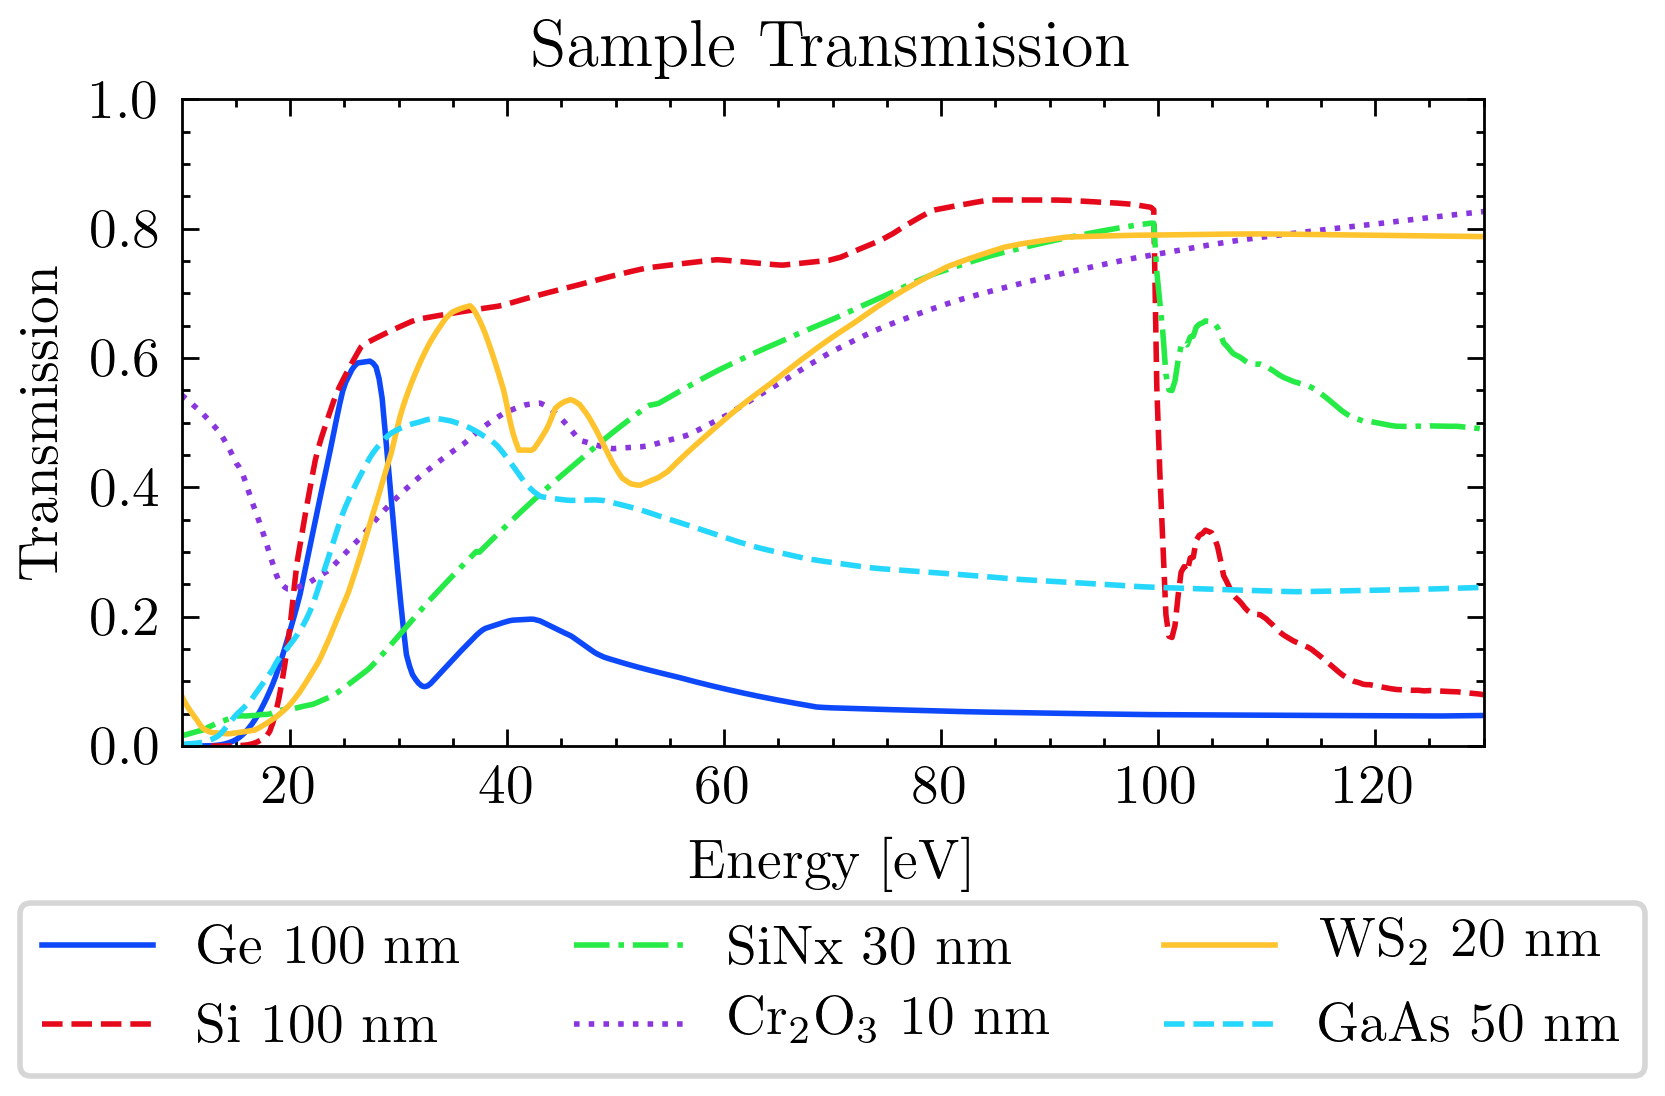
\includegraphics[width=0.75\textwidth]{figures/chap3/Sample_trans_CXRO.png}
	\caption{Calculated XUV transmission of various materials. Data from \cite{gulliksonCXROXRayInteractions}.}
	\label{fig:Sample_trans_CXRO}
	% figure generated using \PythonScripts\CXRO\test\CXRO.py
\end{figure}

There are several sample requirements for a successful condensed matter transient absorption experiment. First and foremost, the sample needs to have an absorption edge within the bandwidth of the XUV source. Second, the material must be the correct thickness for a transmission measurement, given the signal to noise of the appratus. If the material is too thick, the ground state will absorb most of the XUV flux and the resulting spectrum will be too close to the noise floor of the apparatus. If it is too thin, the laser-induced change of the ground state (on the order of $1-10\%$) will be lost in the noise. As a general guideline, a sample that absorbs 50\% at the spectral feature of interest provides a good compromise between these conflicting requirements. \cref{fig:Sample_trans_CXRO} plots the expected transmission of several materials, calculated from the atomic scattering factors \cite{gulliksonCXROXRayInteractions}. A typical sample will be on the order of 10 - 200 nm thick, depending on the material.

Next, the sample needs to be excitable using laser sources present in our lab (i.e., ultrafast pulses with wavelengths between 800 nm and a couple of microns). To minimize the slow build up of heat (on the order of seconds) and laser-induced damage, the sample needs to be rastered through the laser focus as the experiment is performed. This rastering method necessitates both a large clear aperture ($\sim$ 1 mm$^2$ - 1 cm$^2$) and good sample uniformity. Samples that meet the above thickness and clear aperture requirements are extremely delicate, with thicknesses between 5,000 and 100,000 times smaller than their lateral dimensions. As such, one should expect most samples to break before, during and after measurements, and a successful experiment will have a materials pipeline that is capable of producing multiple, consistent samples in a short time frame.

\section{Data Collection}

\begin{figure}
	\centering
	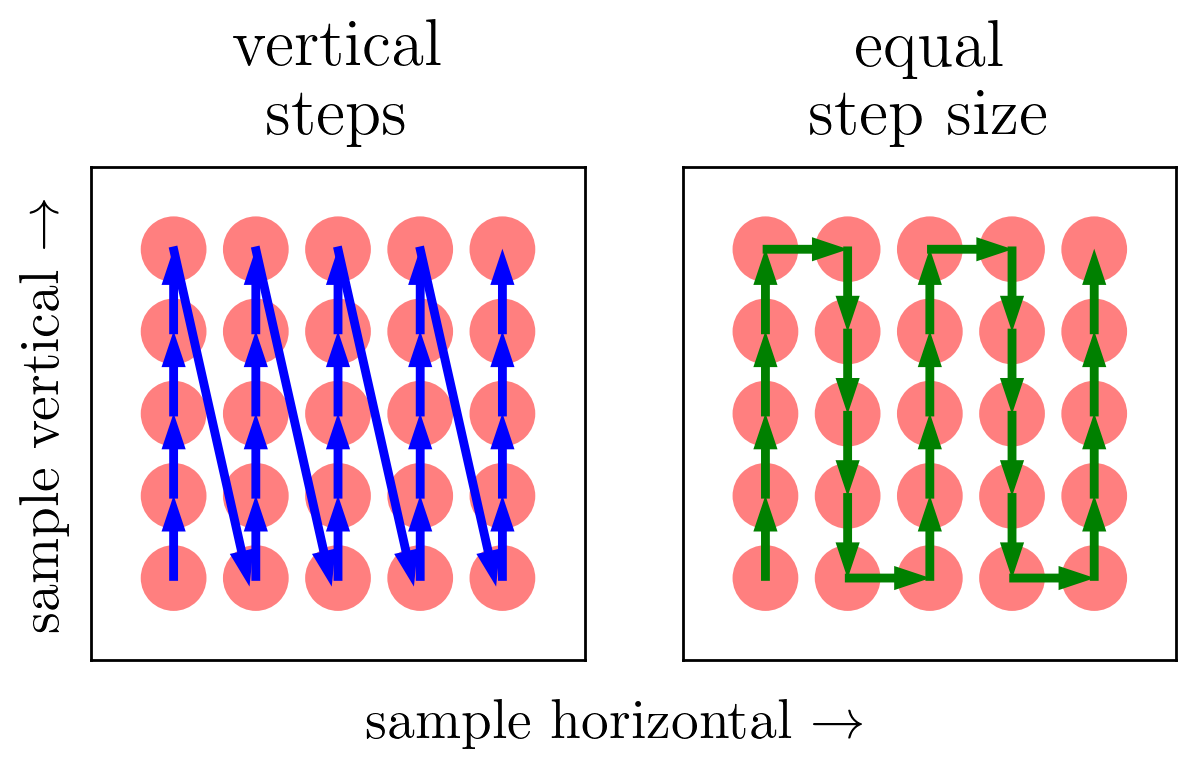
\includegraphics[width=0.75\textwidth]{figures/chap3/Rastering_Methods.png}
	\caption{Schematic of competing raster methods, shown in the sample's reference frame. The clear aperture of the sample is represented by the interior of the black square. The laser propagation is direction is out of the page. The laser focal spots are shown as red circles, and the movement of the sample holder relative to the laser focus is indicated by arrows.}
	\label{fig:Rastering_Methods}
	%figure created using \Python Scripts\rastering\raster_diagram.py
\end{figure}

\begin{figure}
	\centering
	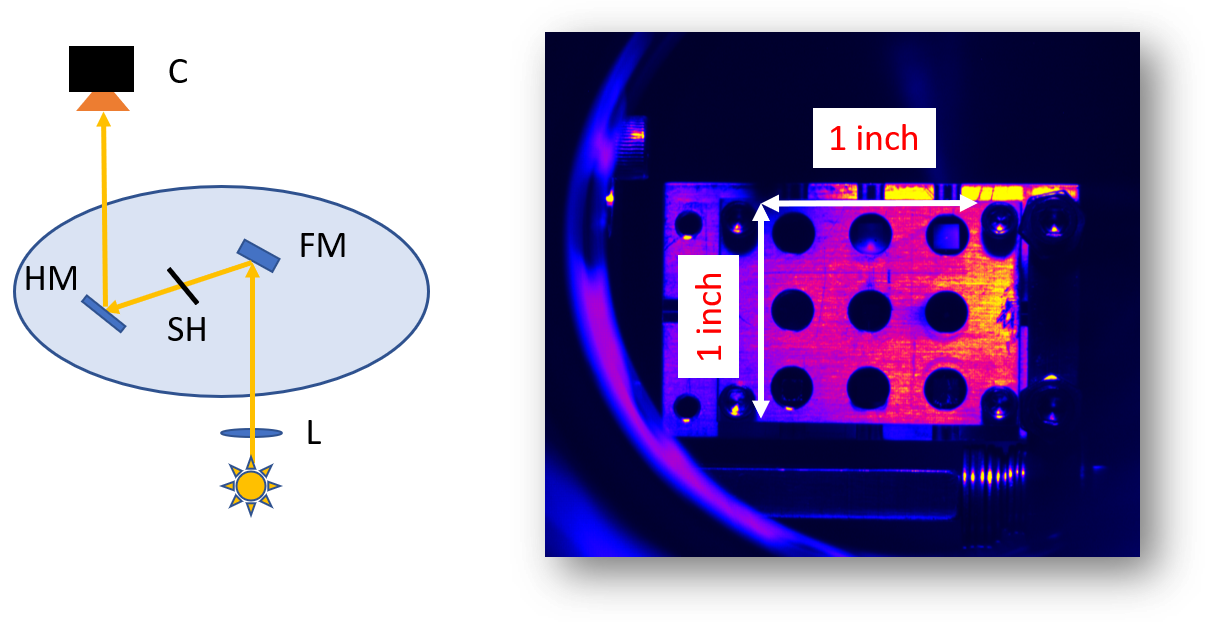
\includegraphics[width=0.75\textwidth]{figures/chap3/sample_holder.png}
	\caption{\textit{In-situ} imaging of the samples within the target chamber. Left: optical setup. C: Si CCD camera, HM: hole mirror, SH: sample holder, FM: flip mirror, L: lens. Right: false color image showing the sample holder with a 3 x 3 grid of 5 mm diameter clear apertures. Samples are held in a clamshell design centered in the clear apertures. Samples are backlit using a flashlight.}
	\label{fig:sample_holder}
\end{figure}

\textbf{talk about general data collection here. i.e., what do you actually record during an experiment?}

The absorbance\footnote{The terms absorbance and optical density are often used interchangably.} $A$ is defined as the negative logarithm of the transmission:
\begin{equation}
A(E) = -\log_{10} \left( T \right) = -\log_{10} \left(\frac{S_{gs}(E)}{S_{vac}(E)} \right).
\label{eqn:absorbance}
\end{equation}

In \cref{eqn:absorbance}, $S_{gs}(E)$ is the XUV spectrum transmitted by the sample in its ground state and $S_{vac}(E)$ is the spectrum without the sample present. Therefore we can measure the sample's ground state absorbance by measuring the harmonic spectrum with and without the sample in the XUV beam.

The \textit{change in absorbance} $\Delta A$ between the ground and excited state which is induced by an IR pulse is therefore:
\begin{equation}
\begin{aligned}
\Delta A(E,\tau) = & A_{sig}(E,\tau) - A_{gs}(E) \\
= & -\log_{10} \left(\frac{S_{sig}(E,\tau)}{S_{vac}(E)} \right) -  \log_{10} \left(\frac{S_{gs}(E)}{S_{vac}(E)} \right) \\
= & -\log_{10} \left(\frac{S_{sig}(E,\tau)}{S_{gs}(E)} \right).
%\Delta A(E,\tau) = -\log_{10} \left(\frac{S_{sig}(E,\tau)}{S_{gs}(E)} \right).
%\label{eqn:delta-OD}
\end{aligned}
\label{eqn:delta-A}
\end{equation}
In \cref{eqn:delta-A}, the signal spectrum $S_{sig}(E,\tau)$ is the spectra that results from an IR pulse hitting the sample, followed by an XUV pulse after a delay of $\tau \equiv t_{XUV} - t_{IR}$. Note that negative delays mean the XUV arrives at the sample before the IR and zero delay indicates temporal overlap of the two pulses. It is assumed that a delay of negative infinity is equivalent to a ground state measurement: $S_{sig}(E,\tau=-\infty) = S_{gs}$.

An ATAS experiment is simply a collection of recorded spectra taken over a range of delay points with otherwise identical experimental conditions. However, we have implemented several techniques to improve the fidelity of our data.

As an extremely nonlinear process, HHG's conversion efficiency is highly dependent on the input laser pointing, peak power, pulse duration, spatial mode, etc. -- all of which are affected by laboratory environmental conditions and the activity of other group members within our lab complex. As a result, the total harmonic yield drifts slowly throughout the course of the experiment. To minimize the effect of this slow drift, we take a ground state spectrum for each delay point. A computer-controlled home-built shutter system blocks the IR laser in the pump arm between measurements (see \cref{fig:beamline_schematic}). Taking back-to-back ground and excited state spectra significantly lowers the harmonic stability requirements; we require stability on the order of twice the exposure time ($\sim$ seconds), rather than the entire experimental run ($\sim$ hours).

Our spectrometer's CMOS camera has a bit depth of 16, corresponding to a maximum value of $2^{16}-1 = 65,535$ counts before saturation. The exposure time is set so that the amplitude of the brightest harmonic on the detector is about 10\% below this limit, which allows for an upward drift in harmonic yield to occur without invalidating the dataset. An exposure time of 3 seconds is typical for a 100 nm Ge sample at 125 Hz (375 laser shots).

Although the Spitfire laser system has a maximum repetition rate of 1 kHz, we perform solid state ATAS experiments at a much lower rate (125 or 250 Hz) by adjusting amplifier's Pockels cell firing rate. The lower repetition rate allows the sample to more fully relax between laser shots, reducing the effects of millisecond thermal processes on our measurements. It also reduces the average power on the sample for a given pulse energy, which lowers the steady state temperature of the sample. On the other hand, it allows us to increase the pulse energy while maintaining a constant average power on the sample.

During the experiment, the sample is rastered across the focus to reduce any deleterious effects of long term uninterrupted laser exposure. During motor movement, the IR beam is blocked with a shutter but the relatively weak XUV beam is allowed to remain on the sample. Each pair of measurements (ground state, excited state) in a given delay scan has a unique position on the sample. Typical step sizes are 200 $\mu$m, which is larger than the measured XUV spot size of $\sim$12 $\mu$m and the IR spot size of $\sim$30 $\mu$m. Two raster schemes are schematically shown in \cref{fig:Rastering_Methods}. The method shown in the left panel produces a sawtooth pattern on the sample. This method gives very accurate positioning, as the vertical motor is almost always approaching the final position from the same direction. However, the diagonal steps are $\sqrt{N^2+1}$ times longer than the vertical steps, where $N$ is the number of vertical steps in the pattern. As a result, there is a bimodal distribution of motor transit times between measurements. If the sample is not fully relaxed between motor movements, this will lead to an inconsistent measurement of the ground state $S_{gs}(E)$. The method shown in the right panel alleviates this problem by requiring equal step sizes. Measurements presented in this work were acquired using the method shown in the right panel.

Before measuring a sample's response for the first time, or after a major optical alignment, a map of the sample must be created. Creating this map serves two purposes: it verifies sample XUV absorption uniformity and it determines the motor coordinates of the sample's clear aperture. To avoid edge effects, the edges of the raster area are chosen to be 200 $\mu$m away from the edge of the clear aperture (see \cref{fig:Rastering_Methods}).

The data collection sequence can be summarized as \textit{excited state $\rightarrow$ ground state $\rightarrow$ move motors}. Details of this sequence are as follows. First, the sample moves to a given raster position and delay wedge position, the IR shutter opens and an excited state measurement is taken. Then, the IR shutter closes and a ground state measurement is taken. Finally, the sample moves to the next raster position as the delay wedge pair moves to the next delay position. The system is programmed to wait for the wedges to become stationary before the next measurement begins.

Note that in this sequence, the time between the $i^{th}$ excited state and $i^{th}$ ground state measurements is equal to the exposure time, but the time between the $i^{th}$ ground state measurement and the $(i+1)^{th}$ excited state measurement is equal to the delay wedge motor transit time\footnote{In this analysis we neglect the role of the XUV-IR delay $\tau$. However, $\tau \sim$ 1 fs - 1 ps, which is neglible compared to the motor transit time $\sim$ 1 s.}. This sequence is preferable to the alternative (\textit{ground state $\rightarrow$ excited state $\rightarrow$ move motors}), as that would result in a delay step size-dependent relaxation time between the $i^{th}$ excited state and the $i+1^{th}$ ground state measurement. Since $\Delta A(E,\tau)$ is calculated between pairs of ground and excited state measurements at a given delay wedge position, the sequence \textit{excited state $\rightarrow$ ground state $\rightarrow$ move motors} is preferred.



To further improve our signal to noise ratio, we average multiple delay scans together. A typical $\Delta A$ measurement will repeat a delay scan between 10 and 50 times. Each delay scan uses the raster points of the previous delay scan so there is a one-to-one mapping of delay to sample position.



damage thresholds, sample thickness, sample uniformity

creating XUV sample maps when we get a new. this allows us to map out the clear aperture of the sample, as well as checking the uniformity of the sample.


\section{Germanium as a Sample}

\begin{figure}
	\centering
	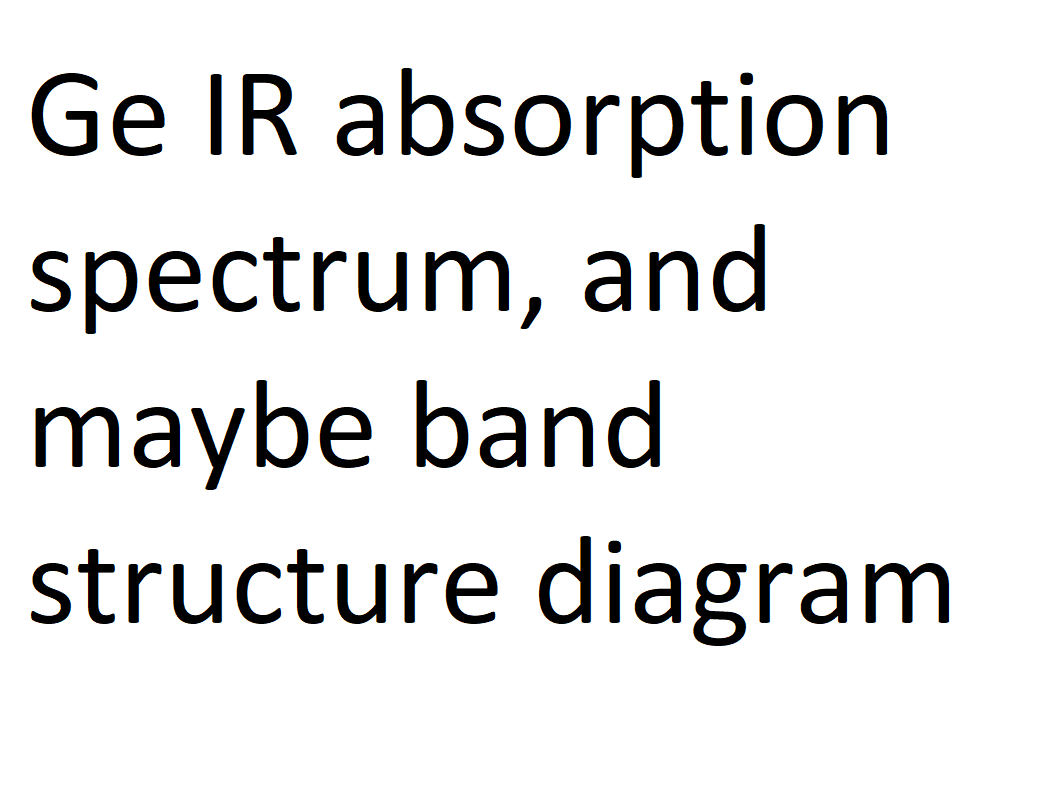
\includegraphics[width=0.5\textwidth]{figures/chap3/Ge_IR_absorption.png}
	\caption{this figure shows the IR absorption of germanium and the band structure, from the literature. (citation)}
	\label{fig:Ge_IR_absorption}
\end{figure}


talk about the germanium sample, why it was chosen as a sample, how it was grown and how thick it was.

\section{Silicon Nitride as a Membrane}

\begin{figure}
	\centering
	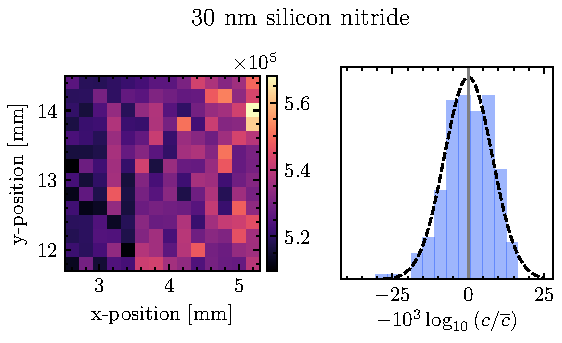
\includegraphics[width=0.75\textwidth]{figures/chap3/nitride_map.png}
	\caption{XUV transmission map of 30 nm silicone nitride freestanding membrane. Left panel: integrated harmonic peaks in the range ?? -- ?? eV. Sample holder motor positions are indicated by x- and y-positions. Right panel: histrogram of logarithmic deviation of counts from the average.}
	\label{fig:nitride_map}
	% figure created using \Python Scripts\Spectrometer\test\rastermap.py
	% dataset: C:\testdata\2019_09_10\4_55_32 PM_nitride_map1
\end{figure}

\begin{figure}
	\centering
	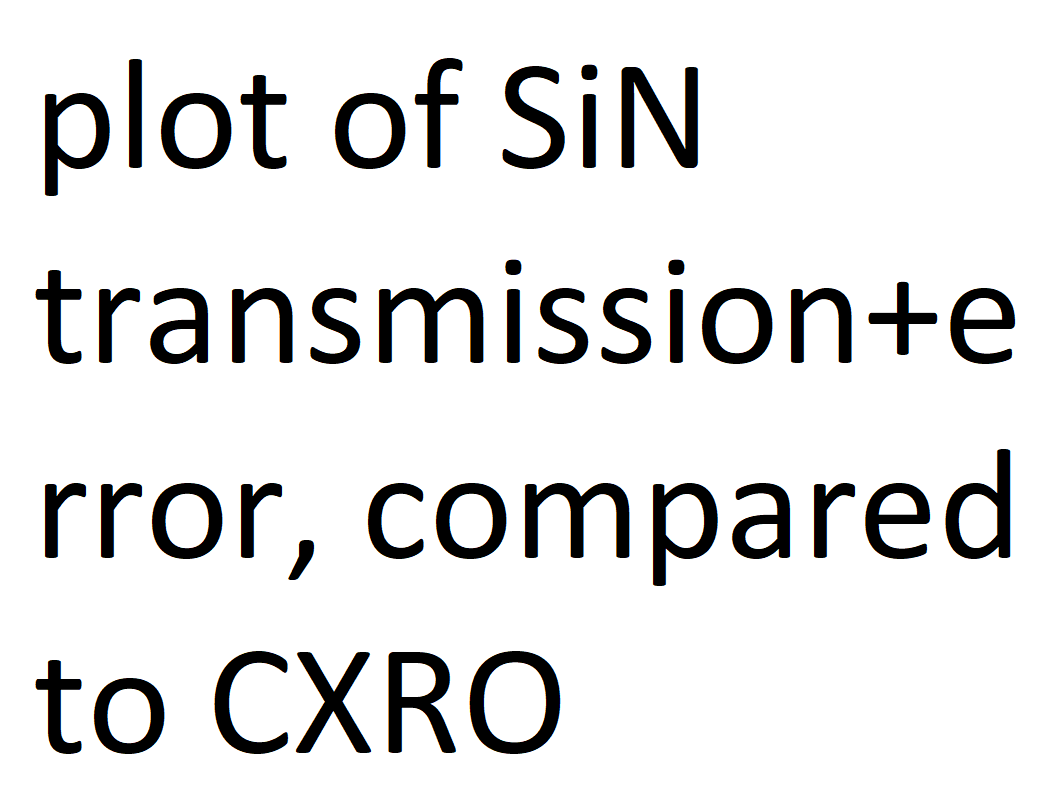
\includegraphics[width=0.5\textwidth]{figures/chap3/Nitride_transmission.png}
	\caption{XUV transmission curve of nitride membrane with error bars. also plotted is CXRO's transmission curve.}
	\label{fig:Nitride_transmission}
\end{figure}

\begin{figure}
	\centering
	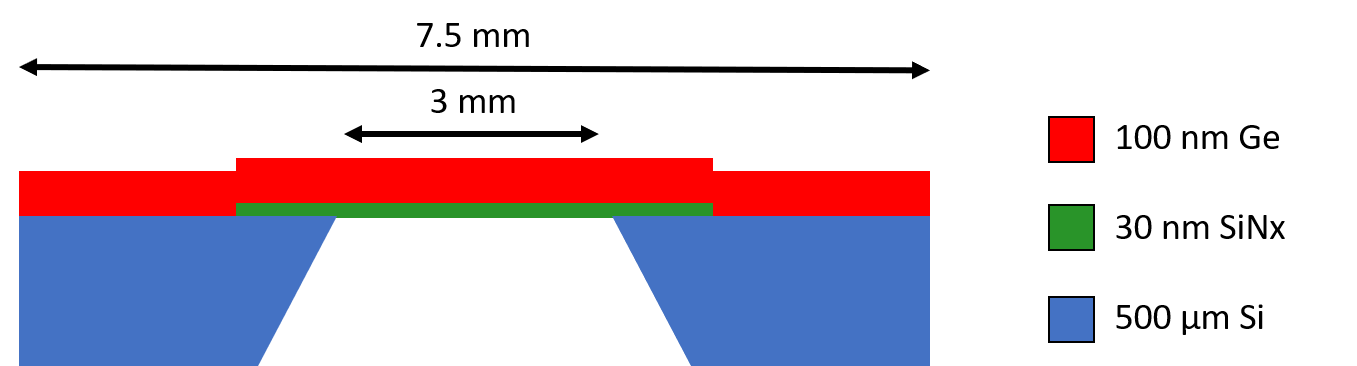
\includegraphics[width=0.75\textwidth]{figures/chap3/Sample_Geometry.png}
	\caption{Cartoon showing the cross section of the free standing sample heterostructure. A 500 $\mu$m thick Si frame supports a 30 nm low stress silicon nitride membrane (Norcada QX7300X), upon which 100 nm of germanium has been deposited. The Si frame has a 3x3 mm$^2$ square clear aperture and a 7.5x7.5 mm$^2$ square external dimension. The taper of the Si frame thickness along the perimeter of the clear aperture forms a knife edge. In an ATAS experiment, the XUV and IR pulses propagate from the top to bottom of the figure.}
	\label{fig:Sample_Geometry}
\end{figure}

Silicon nitride was chosen to be 

why was nitride chosen? large band gap relative to germanium, mechanical robustness, commercial availability and low cost.

measurements of the nitride membrane: maps, histograms - showing how uniform it is. plot the transmission of the nitride membrane.


\section{dialing in the IR parameters}

\begin{figure}
	\centering
	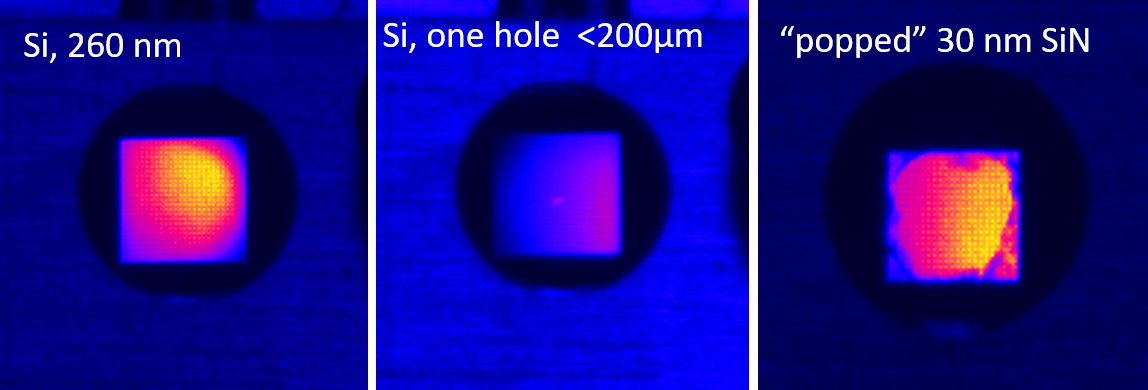
\includegraphics[width=0.75\textwidth]{figures/chap3/sample_damage.png}
	\caption{False color images showing laser drilled freestanding membranes. Left: pristine 260 nm thick Si membrane (Norcada). Middle: same sample, after a performing an IR power scan that exceeded the membrane's damage threshold. A $<$200 $\mu$m hole is visible as a cluster of bright pixels near the center of the membrane. Right: 30 nm SiN membrane after a similar power scan showing a ``popped'' membrane. Note the ragged edges near the clear aperture of the frame are all that remain of the membrane. The apparent brightness gradient across the samples is caused by inconsistent backlighting. Images were taken using the optical setup shown in the left panel of \cref{fig:sample_holder_1}.}
	\label{fig:sample_damage}
\end{figure}

\begin{figure}
	\centering
	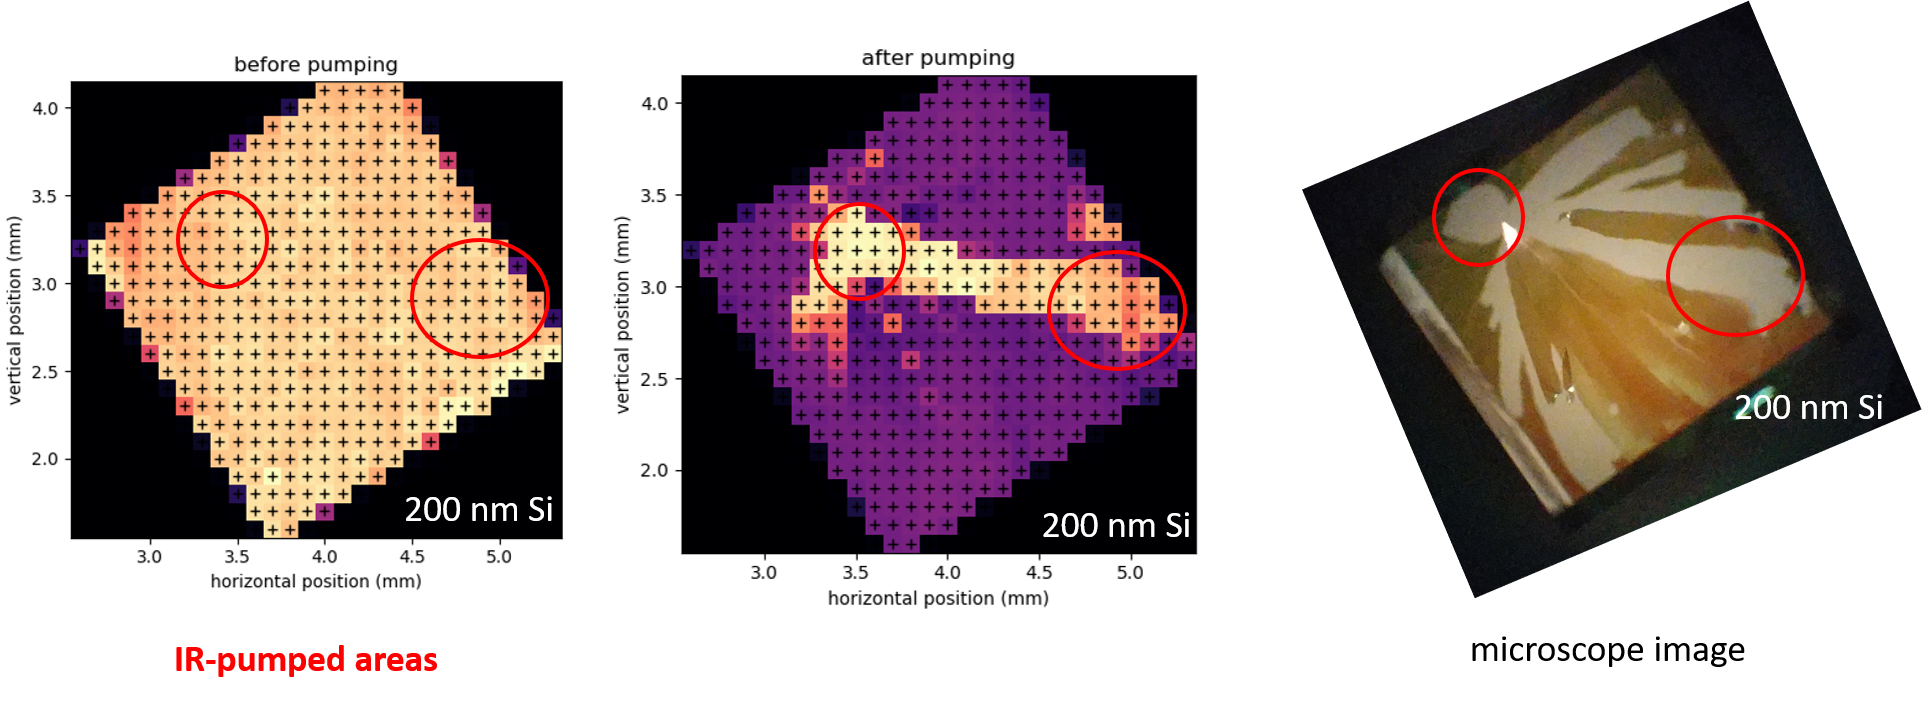
\includegraphics[width=0.75\textwidth]{figures/chap3/Si_damage.png}
	\caption{200 nm silicon}
	\label{fig:Si_damage}
\end{figure}

IR power controlled by waveplate-polarizer pair and monitored during measurements using a photodiode (see \cref{fig:beamline_schematic}). absolute measurements of the average power were taken with a power meter at the completion of the experiment. did intensity scans until the sample was destroyed, then backed off a little bit.


Ge-specific experimental parameters: wavelength, generation conditions, exposure time, MCP settings, rep rate, etc.

show pictures of popped membranes. show delay spectrograms of drilled out samples.

\section{50 nm Ge measurements}
i think we have a dataset or two showing a weak signal.


\section{100 nm Ge measurements}
we went to 100 nm because the 50 nm was too weak.

\begin{figure}
	\centering
	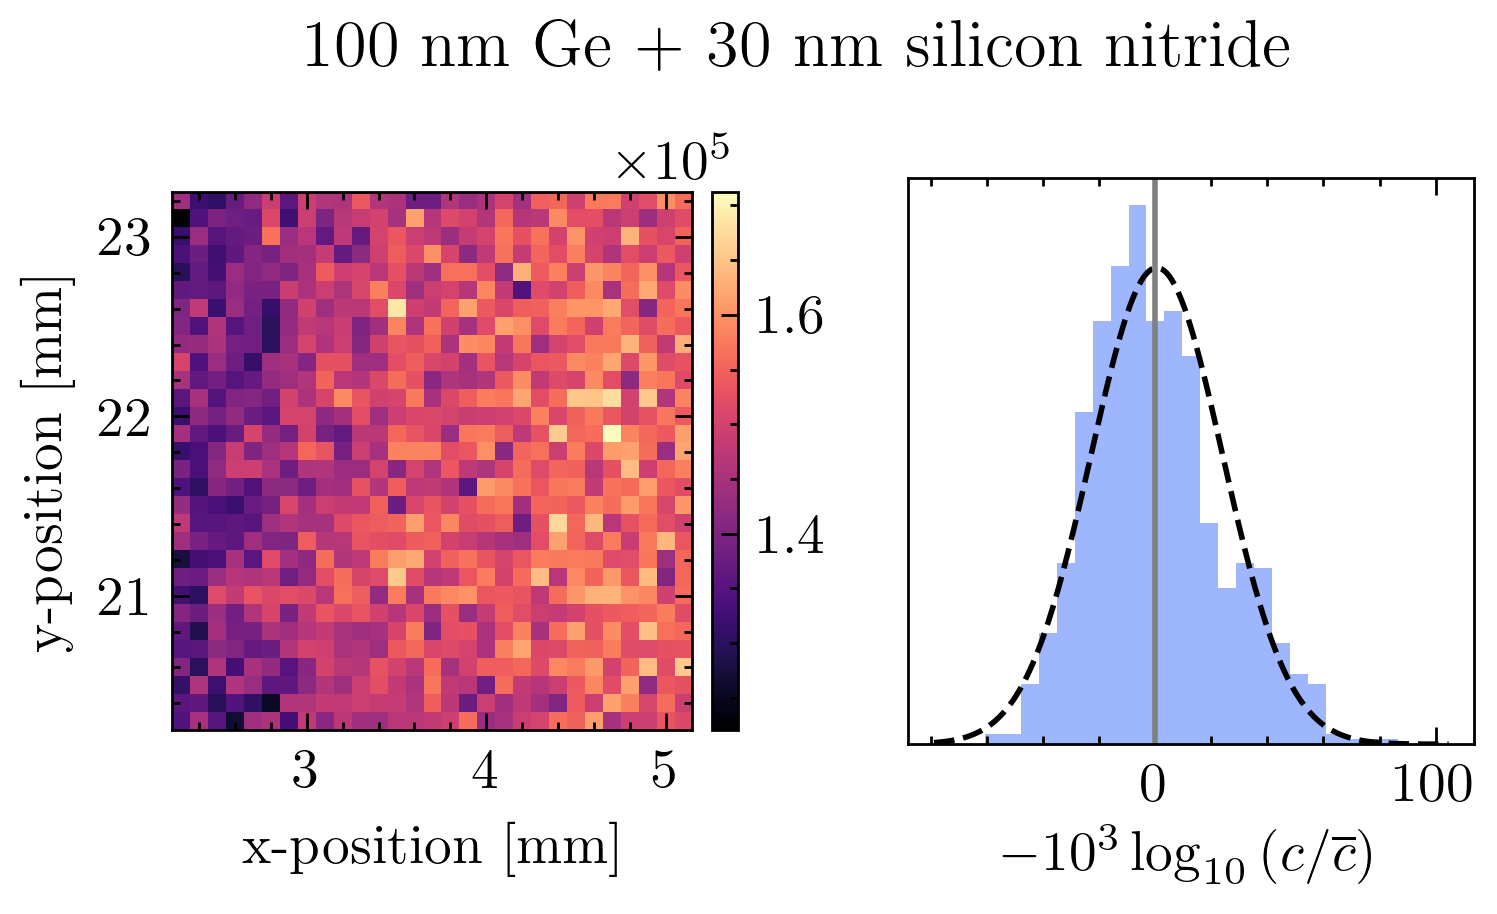
\includegraphics[width=0.75\textwidth]{figures/chap3/Ge_map.png}
	\caption{this is an XUV transmission map of a germanium sample, along with a histogram of the transmission values.}
	\label{fig:Ge_map}
		% figure created using \Python Scripts\Spectrometer\test\rastermap.py
	% dataset: C:\testdata\2019_08_27\11_26_52 AM_Ge7_map1
\end{figure}

\section{Data Processing}

\begin{figure}
	\centering
	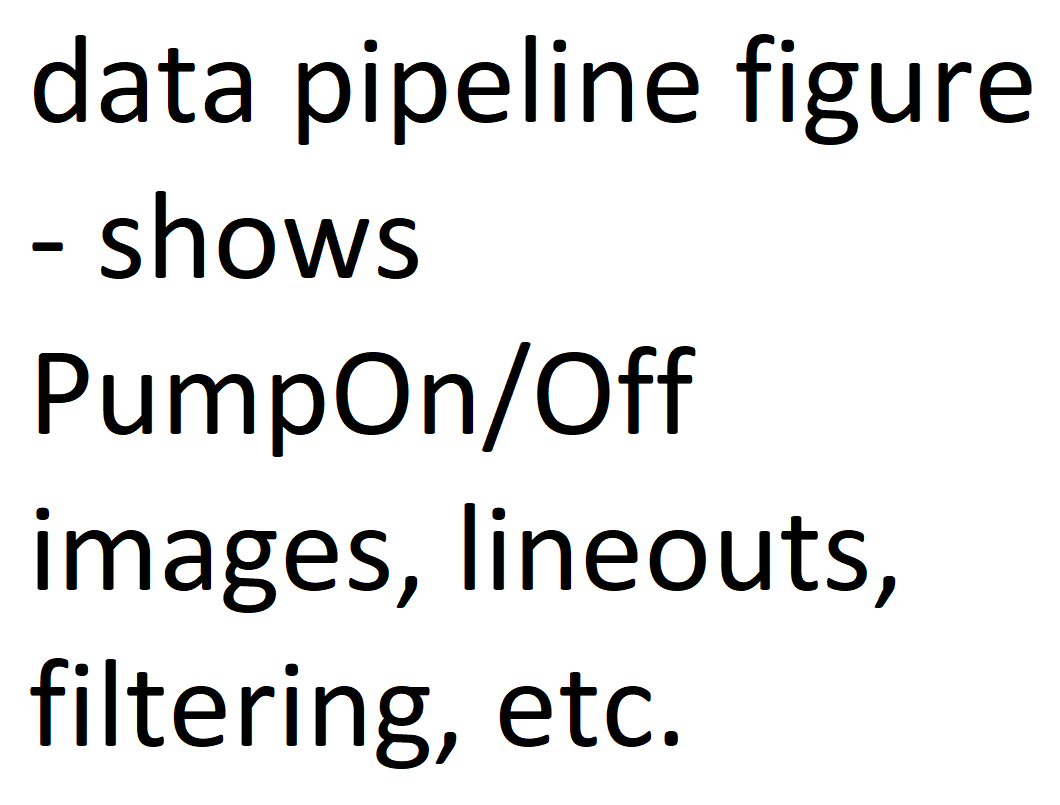
\includegraphics[width=0.5\textwidth]{figures/chap3/Data_Pipeline.png}
	\caption{this figure shows the data processing pipeline. it shows how we start with PumpOn-Off 2D images and transform them into spectrograms. it includes steps like an absorbance (A) calculation, spectral lineouts, frequency filtering and smooth, energy calibration, etc.}
	\label{fig:Data_Pipeline}
\end{figure}

\begin{figure}
	\centering
	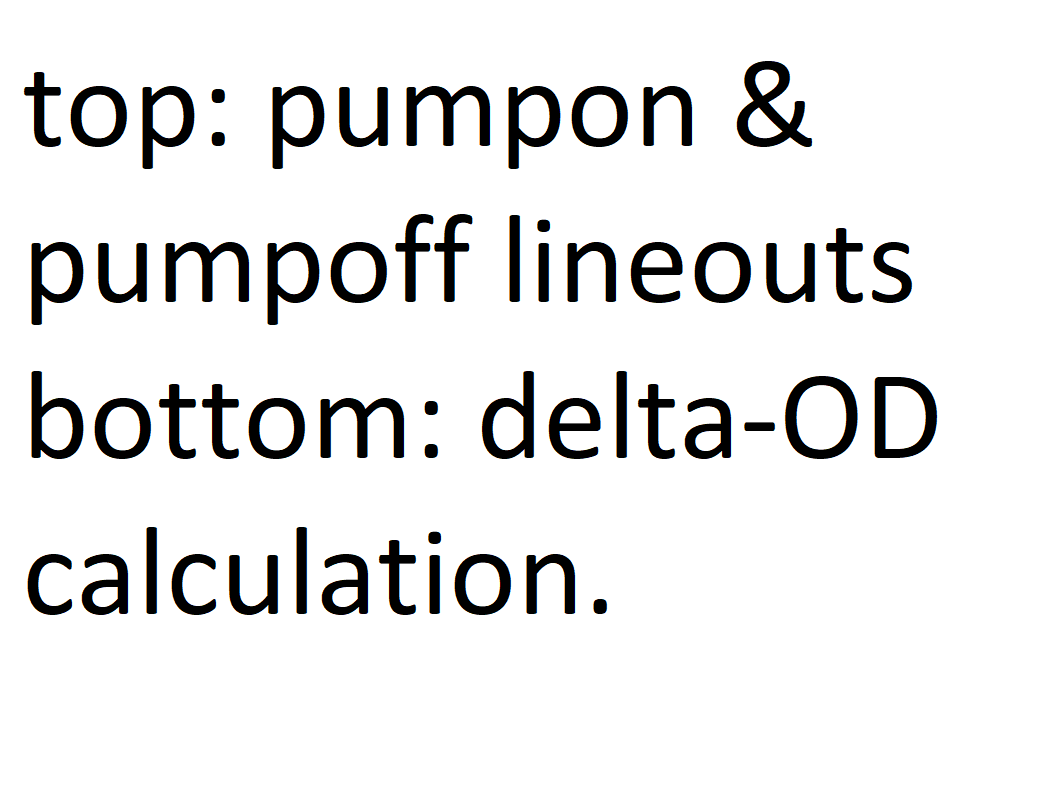
\includegraphics[width=0.5\textwidth]{figures/chap3/PumpOn_vs_PumpOff.png}
	\caption{this figure shows, using real data, a pump off and pump on spectral lineout. in another panel, it shows the $\Delta A$.}
	\label{fig:PumpOn_vs_PumpOff}
\end{figure}

The XUV photon spectrometer utilizes a flat field grating (Hitachi, 1200 l/mm) to spectrally disperse the XUV light. The grating is designed to focus along the spectral axis (horizontal direction) while preserving the spatial profile of the beam (vertical direction). The focus of the grating is incident on a 75 mm diameter imaging quality microchannel plate (MCP) array (Photonis), which converts the XUV photons into electrons via a nonlinear avalanche process with a gain of approximately $10^6 - 10^8$. These electrons strike a phosphor screen, which converts the electrons into visible photons (central wavelength $\sim480$ nm). The visible photons exit the vacuum chamber via a glass feedthrough and are imaged by a lens and CMOS camera (Andor). The result is a two dimensional array of counts, with the horizontal axis representing the spectral content and the vertical axis representing the spatial profile of the beam.

talk about all the steps you use to process the data, starting from the 2d image and ending with the delta-A spectrogram.

mention calibration of spectrometer in passing, 2D image $\rightarrow$ 1D spectrum


